\documentclass[a4paper,12pt]{article}

% Paquetes básicos
\usepackage[utf8]{inputenc}
\usepackage[T1]{fontenc}
\usepackage[spanish]{babel}
\usepackage{graphicx}
\usepackage{xcolor}
\usepackage{lipsum}
\usepackage{geometry}
\geometry{top=3cm, bottom=3cm, left=2.5cm, right=2.5cm}

% Paquetes para diseño
\usepackage{titlesec}
\usepackage{fancyhdr}
\usepackage{amsmath}
\usepackage{amssymb}
\usepackage{hyperref}
\usepackage{float}

% Paquetes para el entorno lstlisting
\usepackage{listings}
\usepackage{inconsolata}

% Paquete para diagramas
\usepackage{tikz}
\usetikzlibrary{shapes, arrows.meta, positioning}

% Paquete para fondo
\usepackage{background}

% Configuración de lstlisting
\lstset{
    language=Python,
    basicstyle=\ttfamily\small,
    keywordstyle=\color{blue}\bfseries,
    stringstyle=\color{teal},
    commentstyle=\color{gray}\itshape,
    numbers=left,
    numberstyle=\tiny\color{gray},
    backgroundcolor=\color{black!5},
    frame=single,
    rulecolor=\color{black!50},
    breaklines=true,
    captionpos=b,
    showstringspaces=false
}

% Configuración de título
\titleformat{\section}{\normalfont\Large\bfseries}{\thesection}{1em}{}

% Información del documento
\title{
    \vspace{-2cm}
    
\includegraphics[width=0.3\textwidth]{images/fccee.jpg} \\ % Cambia el logo si es necesario
    \LARGE Ingeniería Informática + ADE\\
    \large Universidad de Granada (UGR)\\[1cm]
}
\author{\textbf{Autor:} Ismael Sallami Moreno}
\date{\textbf{Asignatura:} Resúmenes de Contabilidad Financiera I Tema 4: Otras operaciones de la actividad corriente de la empresa}

% Configuración del fondo
\backgroundsetup{
    scale=1,
    color=black,
    opacity=0.2,
    angle=0,
    position=current page.south,
    vshift=0pt,
    hshift=0pt,
    contents={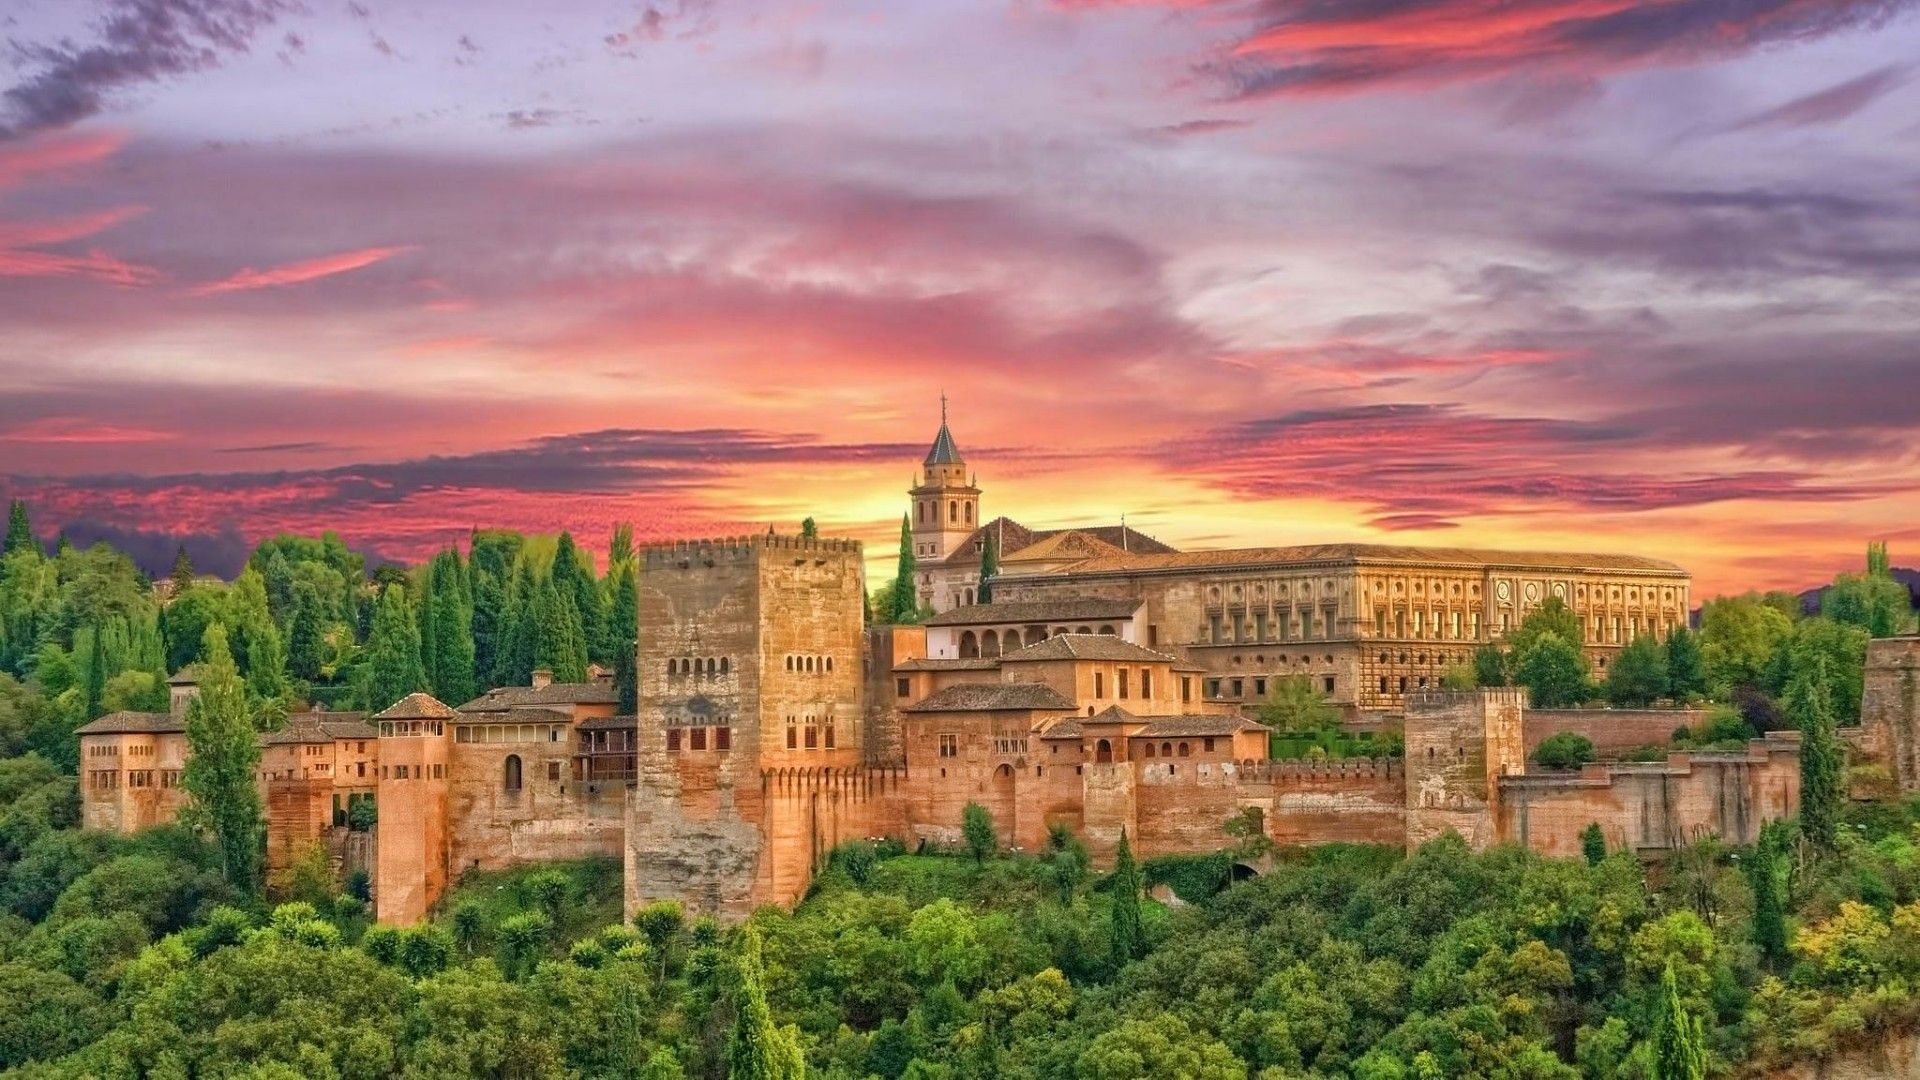
\includegraphics[width=\paperwidth,height=\paperheight,keepaspectratio]{images/granada.jpg}}
}

% Configuración del encabezado y pie de página
\usepackage{times}
\pagestyle{fancy}
\fancyhf{}
\fancyhead[L]{\textbf{\textsf{\leftmark}}}
\fancyhead[R]{\textbf{\textsf{\thepage}}}
\fancyfoot[C]{\thepage}

% Inicio del documento
\begin{document}

% Portada
\maketitle
\thispagestyle{empty}

\begin{center}
    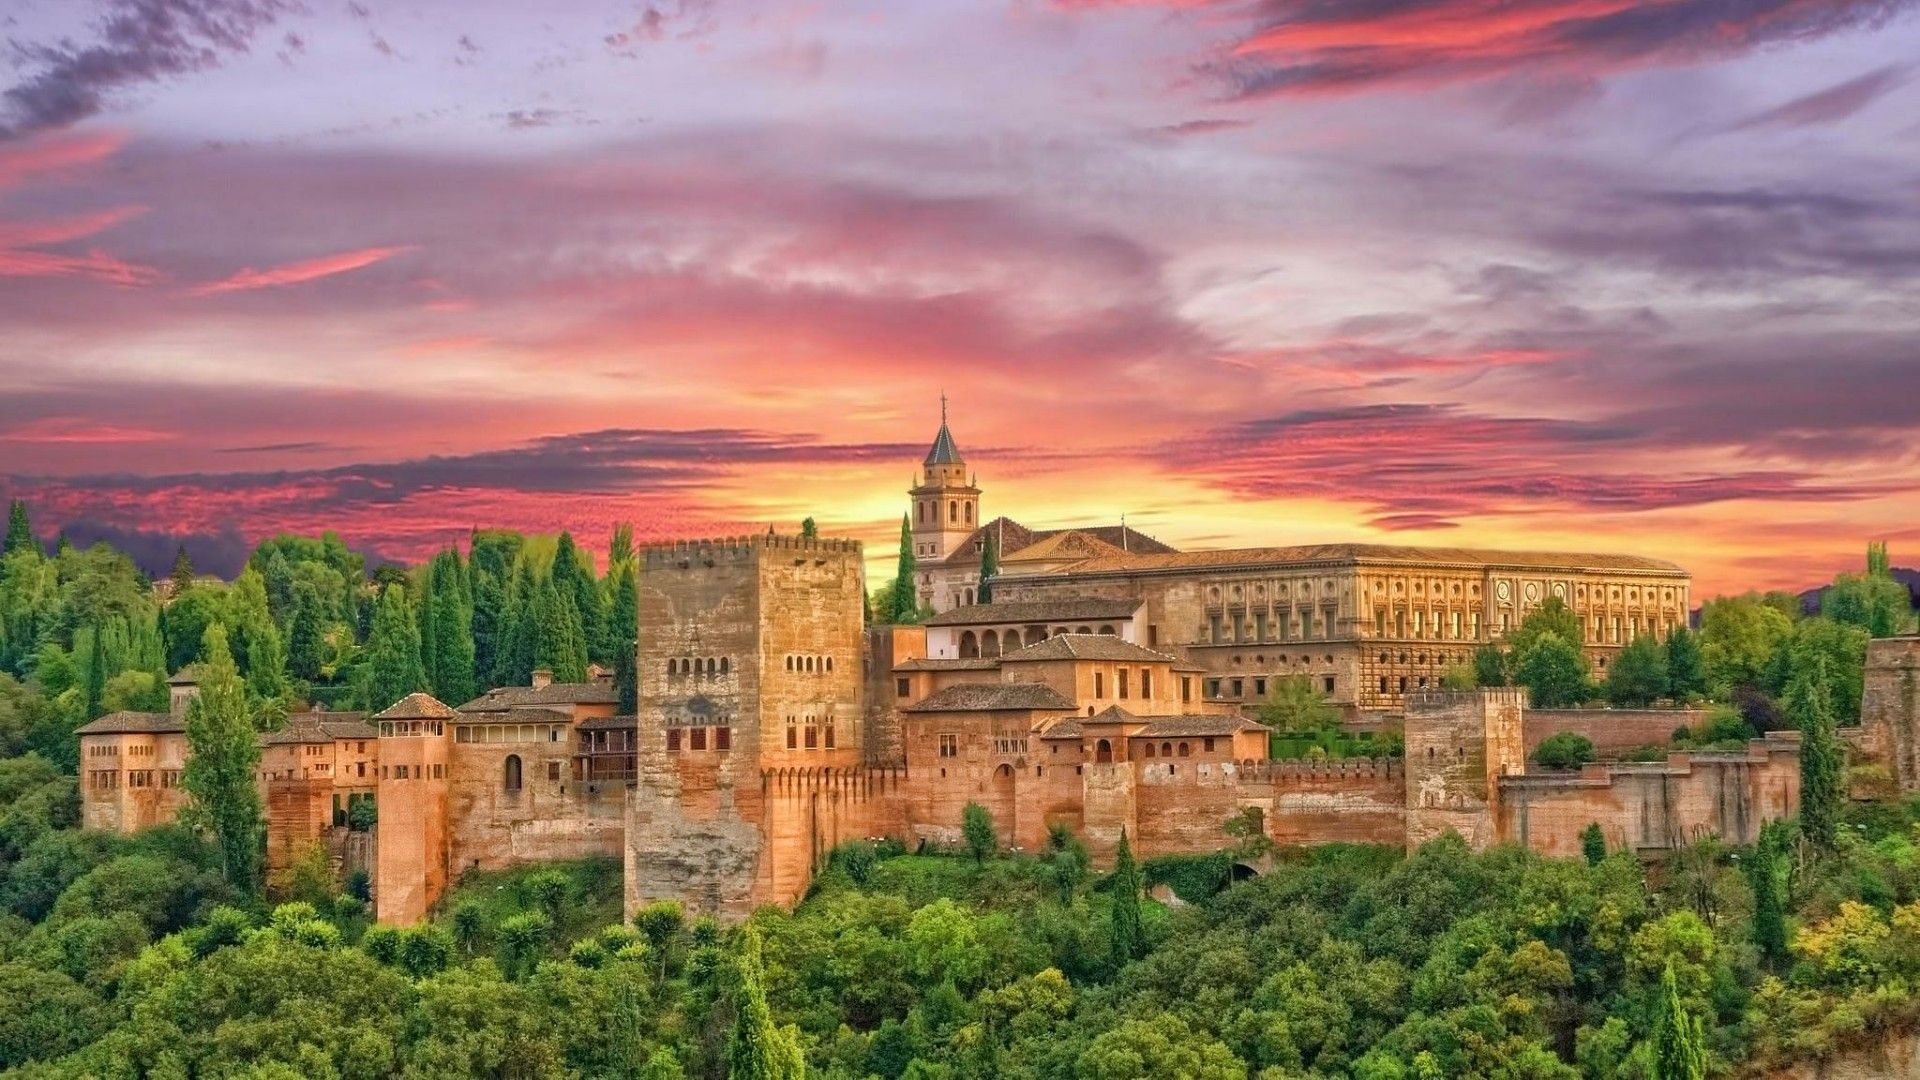
\includegraphics[width=\textwidth,height=0.4\textheight,keepaspectratio]{images/granada.jpg} \\ % Añade tu imagen de fondo
    \vfill
\end{center}

\newpage

% Índice (opcional)
\tableofcontents
\newpage

\section{Gastos e Ingresos: definición y criterios de reconocimiento}

\begin{itemize}
    \item Deben de cumplir con el principio de devengo.
    \item Considerar la prioridad entre la corriente real de bienes y servicios frente a la financiera.
\end{itemize}

\subsection{Ingresos}
Definición: incrementos del PN de la empresa durante el ejercicio económico, en forma de salida o disminución en el valor de los activos, o aumento en el valor de los pasivos, siempre que no tenga su origen en aportaciones de los socios o propietarios.

\subsection{Gastos}
Definición: decrementos del PN de la empresa durante el ejercicio económico, en forma de salidas o disminuciones en el valor de los activos, o aumento en el valor de los pasivos, siempre que no tenga su origen en distribuciones a los socios o propietarios.

\subsection{Criterios de reconocimiento}
El registro de los elementos procederá cuando cumpliéndose con la definición de los mismos, se cumplan los criterios de probabilidad en la obtención o cesión de recursos que incorporen beneficios o rendimientos a la empresa y su valor pueda determinarse con cierto grado de fiabilidad.

\subsection{Gastos en Ingresos que se registran en la cuenta de resultados}

\subsubsection{Gastos}
\begin{itemize}
    \item Grupo 6
    \item Al cierre del ejercicio se abonan con carga a la cuenta 129.
    \item Excepto si funcionan como ingresos:
    \begin{itemize}
        \item 606: descuento sobre compras por pronto pago.
        \item 608: devoluciones de compras y operaciones similares.
        \item 609: rappels sobre compras.
    \end{itemize}
    \item Excepto las cuentas de la variación de existencias (610, 611, 612) que pueden tener sado deudor o acreedor.
\end{itemize}

\subsubsection{Ingresos}
\begin{itemize}
    \item Grupo 7
    \item Al cierre del ejercicio se cargan con abono a la cuenta 129.
    \item Excepto si funcionan como gastos:
    \begin{itemize}
        \item 706: descuento sobre ventas por pronto pago.
        \item 708: devoluciones de ventas y operaciones similares.
        \item 709: rappels sobre ventas.    
    \end{itemize}
    \item Excepto las cuentas de la variación de existencias (71, 710, 713) que pueden tener sado deudor o acreedor.
\end{itemize}

\subsection{Gastos e Ingresos que se imputan directamente al PN}

Estos no pasan por la cuenta de resultados.
\begin{itemize}
    \item Gastos Grupo 8: al cierre del ejercicio se abonan con cargo a las cuentas del subgrupo 13.
    \item Ingresos Grupo 9: al cierre del ejercicio se cargan con abono a las cuentas del subgrupo 13.
\end{itemize}

\subsection{Criterios de reconocimiento y valoración de los Ingresos}

Una empresa reconocerá los ingresos por ventas y prestaciones de servicios cuando se produzca la transferencia del control de los bienes o servicios al cliente.\\
El criterio de transferencia consiste en realizar diversas operaciones contractuales a medida que pasa el tiempo, en función de los respectivos valores razonables.

\subsubsection{Etapas del registro contable de ingresos}

\begin{figure}[H]
    \centering
    \begin{tabular}{|p{6cm}|p{6cm}|}
    \hline
    \textbf{ETAPAS} & \textbf{OBJETIVO} \\ \hline
    Etapa 1. Identificar el contrato con el cliente & Comprobar que se trata de un contrato a efectos NIIF-UE 15 \\ \hline
    Etapa 2. Identificar en el contrato las obligaciones individuales & Distinguir compromisos de transferencia al cliente de bienes o servicios \\ \hline
    Etapa 3. Determinar el precio global de la transacción & Cuantificar la cantidad global a la que empresa espera tener derecho a recibir a cambio \\ \hline
    Etapa 4. Distribuir el precio entre las obligaciones & Asignar a cada obligación una parte del precio global, en función de precios individuales \\ \hline
    Etapa 5. Reconocer ingresos & Registrar ingresos según se vayan cumpliendo las obligaciones. \\ \hline
    \end{tabular}
    \caption{Etapas y objetivos relacionados}
\end{figure}

\newpage
\section{Contabilización de las retribuciones al personal}

Cuentas que reflejan las relaciones entre empresa y trabajadores:
\begin{itemize}
    \item (460) <<Anticipo de remuneraciones.>>
    \item (465) <<Remuneraciones pendientes de pago.>>
    \item (466) <<Remuneraciones mediante sistemas de aportación definida pendientes de pago.>>
\end{itemize}

Estas cuentas tienen la contrapartida en las cuentas del subgrupo 64:
\begin{itemize}
    \item (640). «Sueldos y salarios»
    \item (641). «Indemnizaciones»
    \item (642). «Seguridad Social a cargo de la empresa»
    \item (643). «Retribuciones a l/p mediante sistemas de aportación definida»
    \item (644). «Retribuciones a l/p mediante sistemas de prestación definida»
    \item (645). «Retribuciones al personal mediante instrumentos de patrimonio»
    \item (649). «Otros gastos sociales»
\end{itemize}

Para ver el ejemplo de una nómina pincha \href{https://github.com/ElblogdeIsmael/ElblogdeIsmael.github.io/blob/main/Asignaturas/Tercer%20A%C3%B1o/CF1/Resumenes/Tema4/FCCEE/images/partes_nomina.png}{aquí.}\\

\newpage
El registro contable de las remuneraciones de los trabajadores combina las cuentas de los subgrupos 46 y 64. Los sueldos y salarios se registran en la cuenta (640) \textit{Sueldos y salarios}. La seguridad social, tanto la cuota empresarial como la de los trabajadores, se registra en la cuenta (642) \textit{Seguridad Social a cargo de la empresa}.\\

Para determinar el líquido a percibir por el trabajador, se restan del salario bruto las retenciones del IRPF (cuenta 4750 \textit{Hacienda Pública Acreedora por retenciones practicadas}) y la cuota de la Seguridad Social a cargo del trabajador (junto con la de la empresa en la cuenta 476 \textit{Organismos de la Seguridad Social acreedores}).\\

\section{Servicios Exteriores}
\begin{itemize}
    \item \textbf{620.} «Gastos en investigación y desarrollo del ejercicio»
    \item \textbf{621.} «Arrendamientos y cánones»
    \item \textbf{622.} «Reparaciones y conservación»
    \item \textbf{623.} «Servicios de profesionales independientes»
    \item \textbf{624.} «Transportes»
    \item \textbf{625.} «Primas de seguros»
    \item \textbf{626.} «Servicios bancarios y similares»
    \item \textbf{627.} «Publicidad, propaganda y relaciones públicas»
    \item \textbf{628.} «Suministros»
    \item \textbf{629.} «Otros servicios»
\end{itemize}

\begin{table}[H]
    \centering
    \begin{tabular}{|c|p{7cm}|c|}
    \hline
    \textbf{DEBE} & \textbf{Esquema de registro contable} & \textbf{HABER} \\ \hline
    (62) Servicios exteriores &  &  \\ \hline
    & a (410) Acreedores por prestaciones de servicios por servicios pagados a plazo &  \\ \hline
    & a (57) Tesorería por servicios pagados al contado &  \\ \hline
    & a (14) Provisiones por responsabilidades o grandes reparaciones &  \\ \hline
    & a (529) Provisiones a corto plazo &  \\ \hline
    & a (475) Hacienda pública acreedora por conceptos fiscales por retenciones practicadas &  \\ \hline
    \end{tabular}
    \caption{Contrapartidas del subgrupo 62. «Servicios exteriores».}
\end{table}
    
    
\section{Operaciones Habituales de la empresa en moneda extranjera}
\begin{itemize}
    \item Transacción en moneda extranjera: operación que se liquida en una moneda distinta a la funcional de la empresa.
    \item Moneda funcional: moneda en la que se lleva la contabilidad.
    \item Moneda de presentación: moneda en la que se presentan los estados financieros.
\end{itemize}

Los elementos patrimoniales se diferenciarían según su consideración en:
\begin{itemize}
    \item Partidas Monetarias: son el efectivo, asi como los activos o pasivos que se van a cobrar o pagar.Se incluyen los préstamos y partidas a cobrar, débitos o partidas a pagar y las inversiones que cumplan con los requisitos.
    \item Partidas no monetarias: los activos y pasivos que no se consideran partidas monetarias. Se incluyen los inmovilizados materiales, inversiones inmobiliarias, fondo de comercio y otros inmovilizados intangibles.
\end{itemize}

\subsection{Valoriación y tratamiento contable}

\subsubsection{Valoriación inicial}
\begin{itemize}
    \item Toda moneda extranjera se transformará a moneda funcional a la fecha de la transacción.
    \item La tasa de cambio utilizada será la tasa de cambio de contado entre la moneda funcional y la moneda extranjera en la fecha de la transacción.
    \item Para más información, puedes consultar la \href{https://www.ifrs.org/issued-standards/list-of-standards/ias-21-the-effects-of-changes-in-foreign-exchange-rates/}{Norma Internacional de Contabilidad 21 (NIC 21)}.
\end{itemize}



\begin{figure}[H]
\centering
\begin{tikzpicture}[node distance=1.125cm, every node/.style={fill=white, font=\sffamily\tiny}]
    \node (start) [circle, draw, fill=blue!20] {Operaciones en moneda extranjera};
    \node (trans) [circle, draw, below=of start, fill=blue!20] {Transacciones en moneda extranjera};
    \node (valInit) [rectangle, draw, below left=of trans, fill=green!20] {Valoración inicial};
    \node (valPost) [rectangle, draw, below right=of trans, fill=green!20] {Valoración posterior};
    \node (partMon) [rectangle, draw, below=of valPost, fill=yellow!20] {Partidas monetarias};
    \node (partNoMon) [rectangle, draw, right=of partMon, xshift=1.5cm, fill=yellow!20] {Partidas no monetarias};
    \node (tipoCambio) [rectangle, draw, below=of partMon, yshift=-0.5cm, fill=red!20] {Tipo de cambio al cierre. Diferencias a PyG};
    \node (costeHis) [rectangle, draw, below=of partNoMon, fill=red!20] {Coste histórico/valor razonable};
    \node (convCuentas) [rectangle, draw, right=of trans, xshift=1.125cm, fill=orange!20] {Conversión de las cuentas anuales a la moneda de presentación};
    \node (difPatrimonio) [rectangle, draw, below=of convCuentas, fill=purple!20] {Diferencias a patrimonio neto};

    \draw [arrows = -{Triangle[angle=60:6pt]}] (start) -- (trans);
    \draw [arrows = -{Triangle[angle=60:6pt]}] (trans) -- (valInit);
    \draw [arrows = -{Triangle[angle=60:6pt]}] (trans) -- (valPost);
    \draw [arrows = -{Triangle[angle=60:6pt]}] (valPost) -- (partMon);
    \draw [arrows = -{Triangle[angle=60:6pt]}] (valPost) -- (partNoMon);
    \draw [arrows = -{Triangle[angle=60:6pt]}] (partMon) -- (tipoCambio);
    \draw [arrows = -{Triangle[angle=60:6pt]}] (partNoMon) -- (costeHis);
    \draw [arrows = -{Triangle[angle=60:6pt]}] (trans) -- (convCuentas);
    \draw [arrows = -{Triangle[angle=60:6pt]}] (convCuentas) -- (difPatrimonio);
\end{tikzpicture}
\caption{Tratamiento contable moneda extranjera}
\end{figure}

\subsubsection{Valoración posterior}

\begin{itemize}
    \item Se valorará aplicando el tipo de cambio de cierre.
    \item Las partidas monetarias valoradas inicialmente a coste histórico se valorarán aplicando el tipo de cambio de la fecha de transacción.
    \item Las valoradas a valor razonable se valorarán aplicando el tipo de cambio de la fecha de determinación del valor razonable.
\end{itemize}

\section{Periodificación de gastos e ingresos del ejercicio}

\begin{itemize}
    \item Reflejan la regularización contable.
    \item Objetivo: separar la parte que es consumida en el ejercicio de la que no lo es.
    \item Los gastos e ingresos deben ser reconocidos en el periodo en el que se devengan, independientemente de cuándo se realicen los pagos o cobros.
    \item La periodificación permite una correcta asignación temporal de los gastos e ingresos, mejorando la precisión de los estados financieros.
\end{itemize}

Para más información, puedes consultar la \href{https://www.ifrs.org/issued-standards/list-of-standards/ias-1-presentation-of-financial-statements/}{Norma Internacional de Contabilidad 1 (NIC 1)}.

\section{Información a suministrar en las cuentas anuales}
\begin{itemize}
    \item Importe neto de la cifra de negocios. Esta se calcula restando a las ventas de bienes y servicios el importe de los descuentos y el IVA (y otros impuestos).
    \item Componentes de la misma:
    \begin{itemize}
        \item Positivos: derechos derivados de contratos con clientes.
        \item Negativos:
        \begin{itemize}
            \item Devoluciones de ventas.
            \item Rappels sobre ventas o prestaciones de servicios.
            \item Descuentos por pronto pago fuera de factura.
        \end{itemize}
    \end{itemize}
\end{itemize}

Enlace a imágenes de la cuenta de pérdidas y ganancias y demás: \href{https://github.com/ElblogdeIsmael/ElblogdeIsmael.github.io/tree/main/Asignaturas/Tercer%20A%C3%B1o/CF1/Resumenes/Tema4/FCCEE/images/figuras}{enlace.}

\section{Cuestionario tipo test}
Para realizar el tipo test del libro pinche \href{https://elblogdeismael.github.io/Asignaturas/Tercer%20A%C3%B1o/CF1/Tests/testT4libro.html}{aquí.}

\end{document}
